\section{Señalamiento original}

    El señalamiento original, ilustrado en la Figura \ref{fig:EJ3_2}, incluye 31 señales en total. La mayoría de las cuales se sitúan cerca de la curva y contra curva principal o próximas a las estaciones. Nombrarlas una a una sería impráctico, pero se pueden destacar a grandes rangos donde se sitúan, que funciones cumplen y cuales descuidan. En primer lugar, todos los finales de vía absolutos se encuentran desprotegidos, así como gran parte de las playas de maniobras. En segundo lugar, el señalamiento prioriza la circulación de las formaciones en una única dirección, dependiendo de cual vía se inspeccione. Esto lleva a concluir, a prior, que el señalamiento esta subdimensionado al punto de no permitir explotar todas las características de la red ferroviaria.
    
    \begin{figure}[H]
    	\centering
    	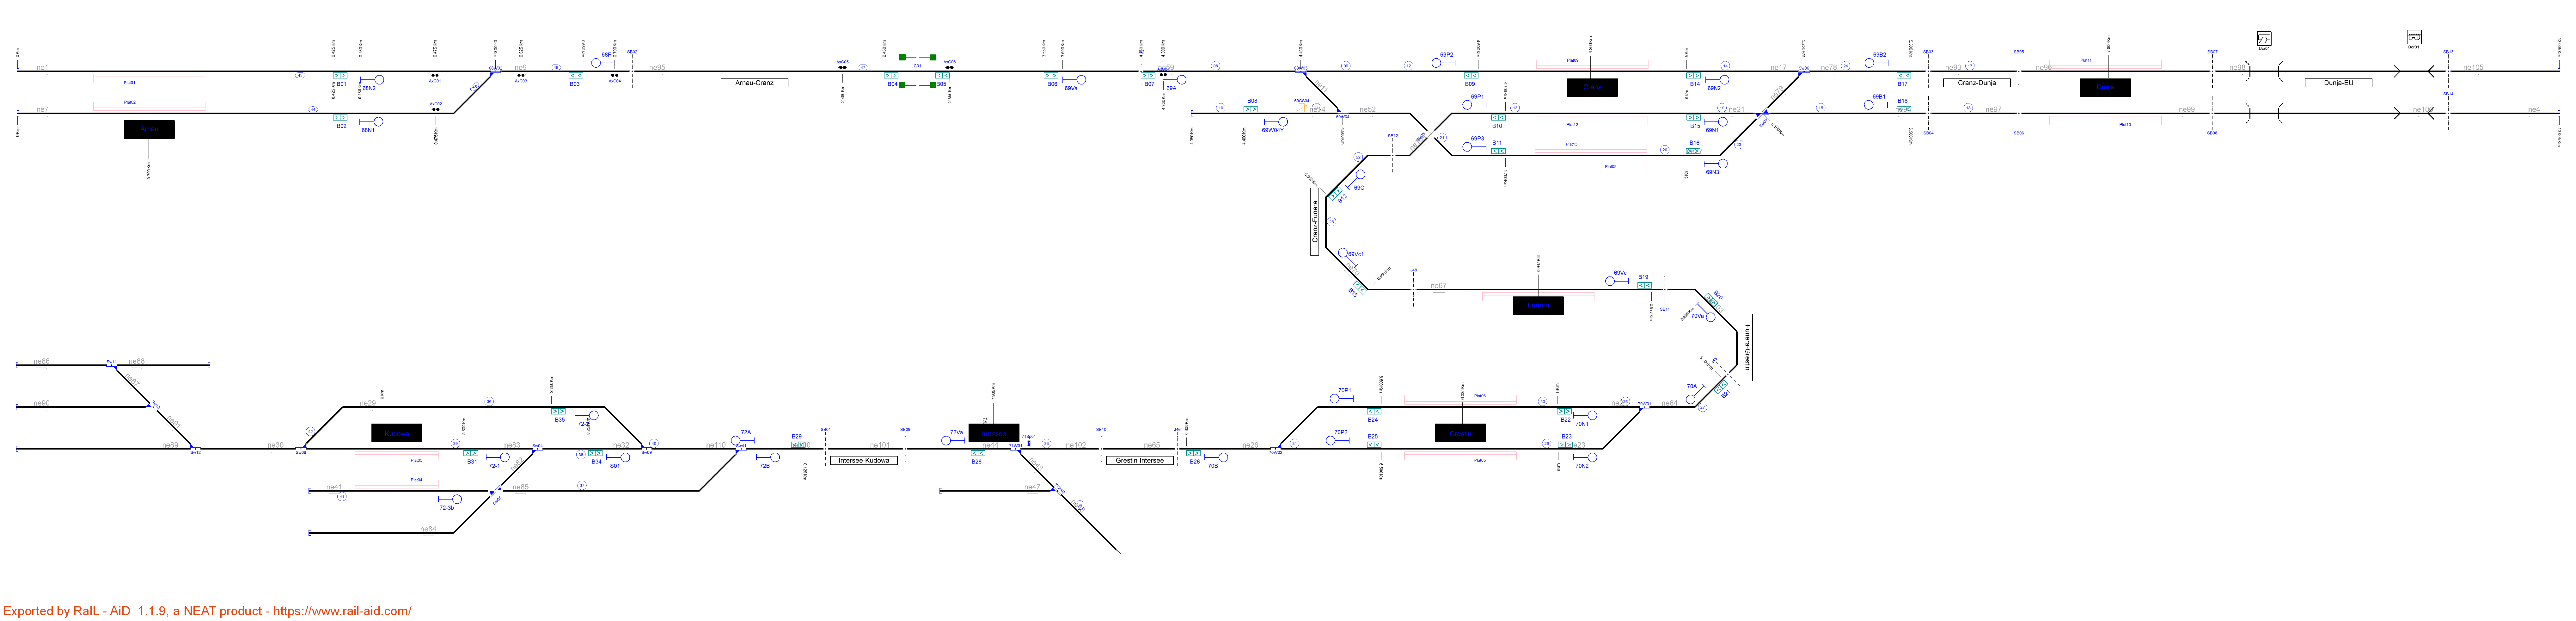
\includegraphics[width=1\textwidth]{resultados-obtenidos/ejemplo3/images/3_original.png}
    	\centering\caption{Señalamiento original del ejemplo 3.}
    	\label{fig:EJ3_2}
    \end{figure}
    
    Estas señales permiten definir hasta un máximo de 33 rutas, todas ellas detalladas en la Tabla \ref{Tab:tabla_original_3}. En una primera inspección, es evidente la ausencia de señalamiento en los límites de la red ferroviaria y en las playas de maniobras. Incluso pueden advertirse alguna situaciones donde las señales otorgarían autoridades ambiguas, lo cual va en contra del principio de claridad. Por ejemplo, la señal 72A podría habilitar una ruta hacia la izquierda de la topología, pero no queda claro que camino tomaría al usar el cambio de vías Sw09, Sw04, Sw08, Sw12, Sw13 y S11; permitiendo hasta 32 posibles caminos.
    
    \begin{table}[H]
        {
        \caption{Tabla de enclavamiento original del ejemplo 3.}
        \label{Tab:tabla_original_3}
        \centering
        \resizebox{1\textwidth}{!}{
            \begin{tabular}{ c c c c c c c }
                \hline	
                    Ruta & Inicio & Final & Cambio & Plataforma & Cruce & netElement \\	
                \hline
                    R$_{01}$ & 68N1 & 69Va & - & - & Lc$_{01}$ & ne$_{7}$-ne$_{95}$\\
                    R$_{02}$ & 68N2 & 69Va & - & - & Lc$_{01}$ & ne$_{1}$-ne$_{95}$\\
                    R$_{03}$ & 69Va & 69A & - & - & - & ne$_{95}$-ne$_{59}$\\
                    R$_{04}$ & 69A & 69N2 & 69W$_{03}^{N}$ & Plat$_{09}$ & - & ne$_{59}$-ne$_{17}$\\
                    R$_{05}$ & 69A & 69N3 & 69W$_{03}^{R}$ & Plat$_{13}$ & - & ne$_{59}$-ne$_{77}$\\
                    R$_{06}$ & 69P2 & 68F & - & - & - & ne$_{17}$-ne$_{9}$\\
                    R$_{07}$ & 69B2 & 69P2 & Sw$_{06}^{N}$ & Plat$_{09}$ & - & ne$_{78}$-ne$_{17}$\\
                    R$_{08}$ & 69B2 & 69P3 & Sw$_{06}^{R}$+Sw$_{07}^{S}$ & Plat$_{13}$ & - & ne$_{78}$-ne$_{77}$\\
                    R$_{09}$ & 69B2 & 69P1 & Sw$_{06}^{R}$+Sw$_{07}^{T}$ & Plat$_{12}$ & - & ne$_{78}$-ne$_{21}$\\
                    R$_{10}$ & 69C & 69N1 & - & Plat$_{12}$ & - & ne$_{70}$-ne$_{21}$\\
                    R$_{11}$ & 69Vc1 & 69C & - & - & -  & ne$_{70}$-ne$_{70}$\\
                    R$_{12}$ & 69Vc & 69Vc1 & - & Plat$_{07}$ & - & ne$_{67}$-ne$_{70}$\\
                    R$_{13}$ & 70Va & 70A & - & - & -  & ne$_{103}$-ne$_{64}$\\
                    R$_{14}$ & 70N2 & 69Vc & - & - & -  & ne$_{23}$-ne$_{67}$\\
                    R$_{15}$ & 70N1 & 69Vc & - & - & - & ne$_{24}$-ne$_{67}$\\
                    R$_{16}$ & 70P1 & 72Va & - & - & - & ne$_{24}$-ne$_{44}$\\
                    R$_{17}$ & 70P2 & 72Va & - & - & - & ne$_{23}$-ne$_{44}$\\
                    R$_{18}$ & 70B & 70N2 & 70W$_{02}^{N}$ & Plat$_{05}$ & - & ne$_{26}$-ne$_{23}$\\
                    R$_{19}$ & 70B & 70N1 & 70W$_{02}^{R}$ & Plat$_{06}$ & - & ne$_{26}$-ne$_{24}$\\
                    R$_{20}$ & 70A & 70P1 & 70W$_{01}^{N}$ & Plat$_{06}$ & - & ne$_{64}$-ne$_{24}$\\
                    R$_{21}$ & 70A & 70P2 & 70W$_{01}^{R}$ & Plat$_{05}$ & - & ne$_{64}$-ne$_{23}$\\
                    R$_{22}$ & 69W04Y & 69N3 & - & Plat$_{13}$ & - & ne$_{14}$-ne$_{77}$\\
                    R$_{23}$ & 72Va & 72A & - & - & - & ne$_{44}$-ne$_{100}$\\
                    R$_{24}$ & 721 & S01 & - & - & - & ne$_{83}$-ne$_{32}$\\
                    R$_{25}$ & 723b & S01 & Sw$_{05}^{T}$ & - & - & ne$_{41}$-ne$_{32}$\\
                    R$_{26}$ & 723b & 72B & Sw$_{05}^{S}$ & - & - & ne$_{41}$-ne$_{100}$\\
                    R$_{27}$ & 722 & 72B & - & - & - & ne$_{29}$-ne$_{100}$\\
                    R$_{28}$ & S01 & 72B & - & - & - & ne$_{32}$-ne$_{100}$\\
                    R$_{29}$ & 69B1 & 69P3 & Sw$_{07}^{T}$ & Plat$_{13}$ & - & ne$_{94}$-ne$_{77}$\\
                    R$_{30}$ & 69B1 & 69P1 & Sw$_{07}^{S}$ & Plat$_{12}$ & - & ne$_{94}$-ne$_{21}$\\
                    R$_{31}$ & 72B & 70B & 71W$_{01}^{N}$ & - & - & ne$_{100}$-ne$_{26}$\\
                    R$_{32}$ & 69P3 & 68F & 69W$_{04}^{R}$ & - & - & ne$_{77}$-ne$_{9}$\\
                    R$_{33}$ & 69P1 & 70Va & - & - & - & ne$_{21}$-ne$_{103}$\\
                \hline
            \end{tabular}
        }
     }
    \end{table}
    
    Todas las rutas abarcan mas de un \textit{netElement}, como por ejemplo la ruta R32 que comienza en la señal 69P3 y finaliza en la señal 68F, atravesando los \textit{netElements} ne77 y ne9, utilizando el cambio de vías 69W04 en posición reversa.